%% kapa: exam=1 round=35 year=2024 period=1 form=A subject=economics subject_ko=경제학원론 seq=1 number=41
%% source: Q-Net 감정평가사 기출문제 (cst00309) artlSeq=5213229 file=raw/1008/5213229/1교시 문제지 원본.pdf
%% conversion: kordoc 4.24.51 -> tools/gen1.py (auto); review=proofread-sonnet; flags=tikz
\begin{question}{41}
( )에 들어갈 내용으로 옳은 것은?
\begin{framedtext}
아래 그림과 같이 두 재화 $X$, $Y$에 대한 갑의 예산선이 $AC$에서 $BC$로 변했을 때, $Y$재 가격이 변하지 않았다면, $X$재 가격은 ( ㄱ )하고, 소득은 ( ㄴ ) 한 것이다.
\begin{center}
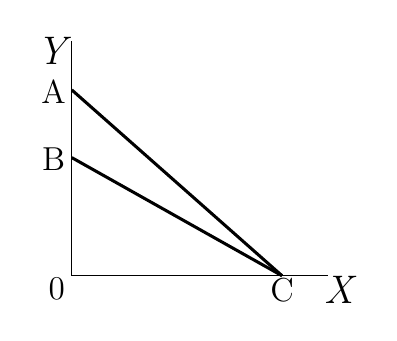
\begin{tikzpicture}[x=0.1mm,y=-0.1mm,font=\small,line width=0.5pt]
\draw (45,10) -- (45,308) -- (370,308);
\draw[line width=1.1pt] (45,72) -- (312,308);
\draw[line width=1.1pt] (45,158) -- (312,308);
\node at (24,22) {\Large\textit{Y}};
\node at (388,326) {\Large\textit{X}};
\node at (26,324) {\large 0};
\node at (22,75) {\large A};
\node at (22,160) {\large B};
\node at (312,326) {\large C};
\end{tikzpicture}
\end{center}
\end{framedtext}
\begin{choices}
  \item ㄱ: 하락, ㄴ: 감소
  \item ㄱ: 하락, ㄴ: 증가
  \item ㄱ: 불변, ㄴ: 감소
  \item ㄱ: 상승, ㄴ: 증가
  \item ㄱ: 상승, ㄴ: 불변
\end{choices}
\end{question}
\answer{1}
